Pada bab ini, akan menunjukkan hasil dari implementasi model. 
\section{Pengaruh Skala Model terhadap Performa model}
Hasil pelatihan model dapat dilihat pada Gambar \ref{fig:model_comparison}.

\begin{figure}[!ht]
    \resizebox{\linewidth}{!}{
        \begin{minipage}{0.3\linewidth}
            \resizebox{\linewidth}{!}{
                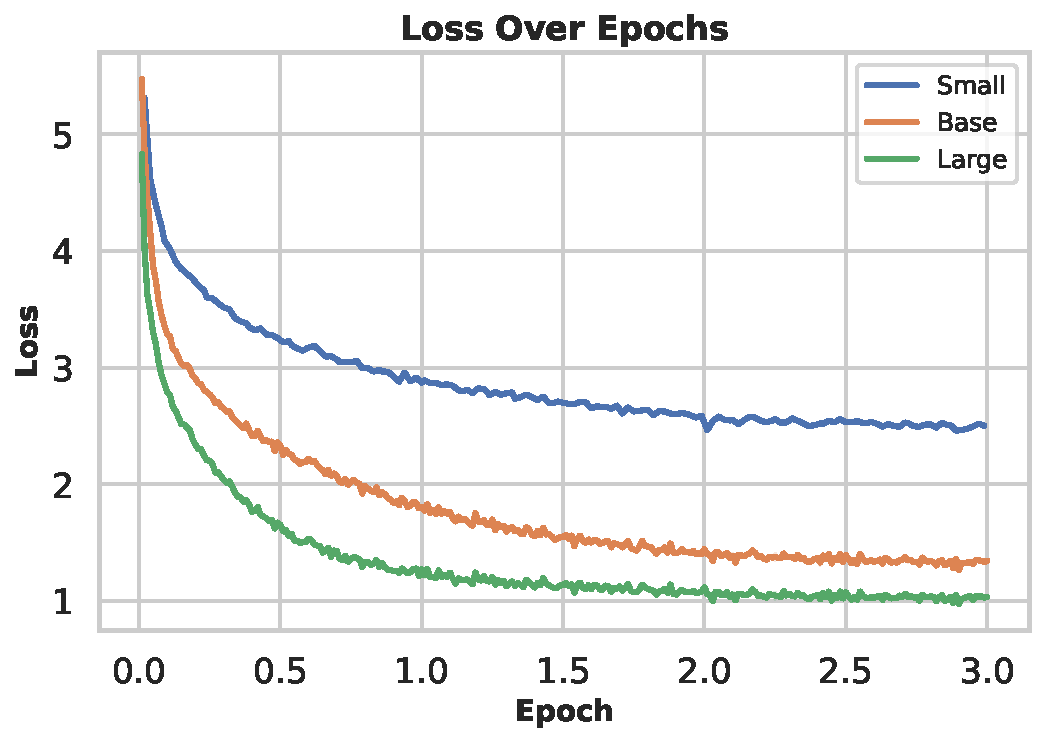
\includegraphics[trim=0 0 0 0,clip]{Figures/loss_plot.pdf}
            }
        \end{minipage}
        \hspace{2pt}
        \begin{minipage}{0.3\linewidth}
            \resizebox{\linewidth}{!}{
                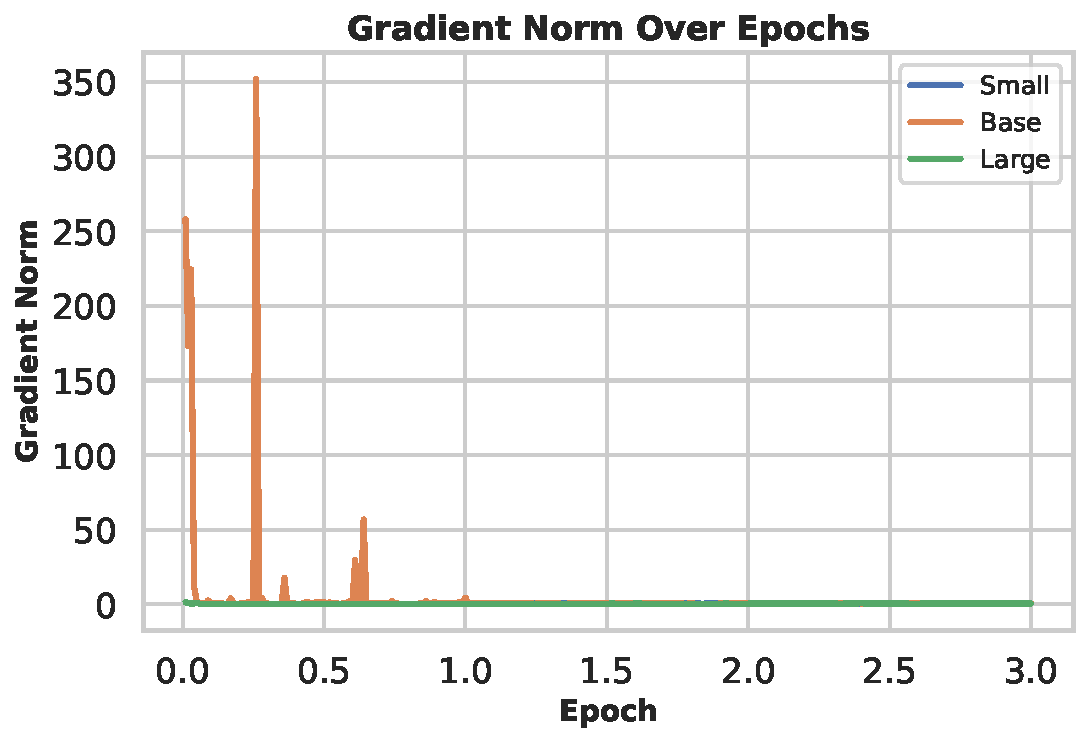
\includegraphics[trim=0 0 0 0,clip]{Figures/grad_norm_plot.pdf}
            }
        \end{minipage}
        \hspace{2pt}
        \begin{minipage}{0.3\linewidth}
            \resizebox{\linewidth}{!}{
                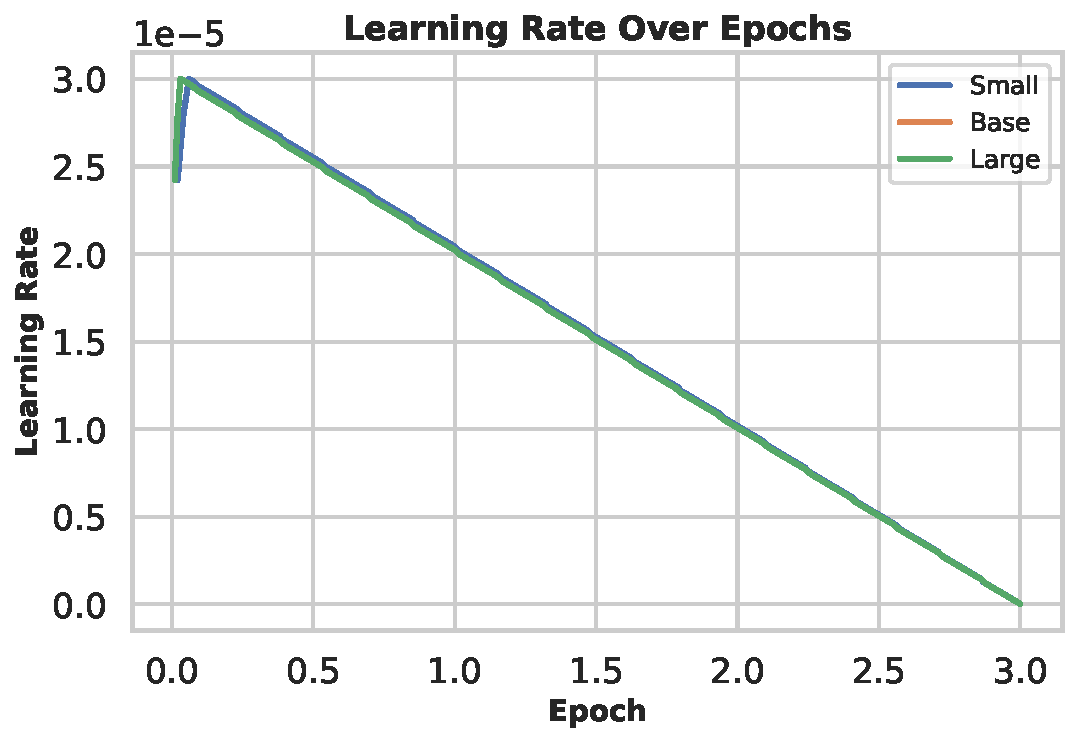
\includegraphics[trim=0 0 0 0,clip]{Figures/learning_rate_plot.pdf}
            }
        \end{minipage}

    }
    % }
    \caption{Evaluasi Proses Pelatihan Model}
    \label{fig:model_comparison}
\end{figure}